\documentclass[tikz,border=12pt]{standalone}
\usepackage[T1]{fontenc}
\usepackage{tgheros}
\usepackage{sfmath}
\usepackage{amsmath,amssymb}
% % \usepackage{fontawesome5} (Removed for publication-grade academic typography) (Removed for publication-grade academic typography)
\usepackage{tikz}
\usetikzlibrary{arrows.meta,positioning,shapes.geometric,fit,backgrounds,calc}
\usepackage{xcolor}

\renewcommand{\familydefault}{\sfdefault}

% Canonical Semantic Palette
\definecolor{structuralnavy}{HTML}{1B2A4A}
\definecolor{measuredteal}{HTML}{168F84}
\definecolor{proposalamber}{HTML}{C98218}
\definecolor{consequencecoral}{HTML}{BD4F2F}
\definecolor{authorityviolet}{HTML}{6550A8}
\definecolor{neutralgray}{HTML}{687386}
\definecolor{navyfill}{HTML}{E8EDF6}
\definecolor{tealfill}{HTML}{E4F6F3}
\definecolor{amberfill}{HTML}{FFF3DC}
\definecolor{coralfill}{HTML}{FAE9E2}
\definecolor{grayfill}{HTML}{F4F6F7}
\definecolor{cardborder}{HTML}{CBD5E1}

\begin{document}
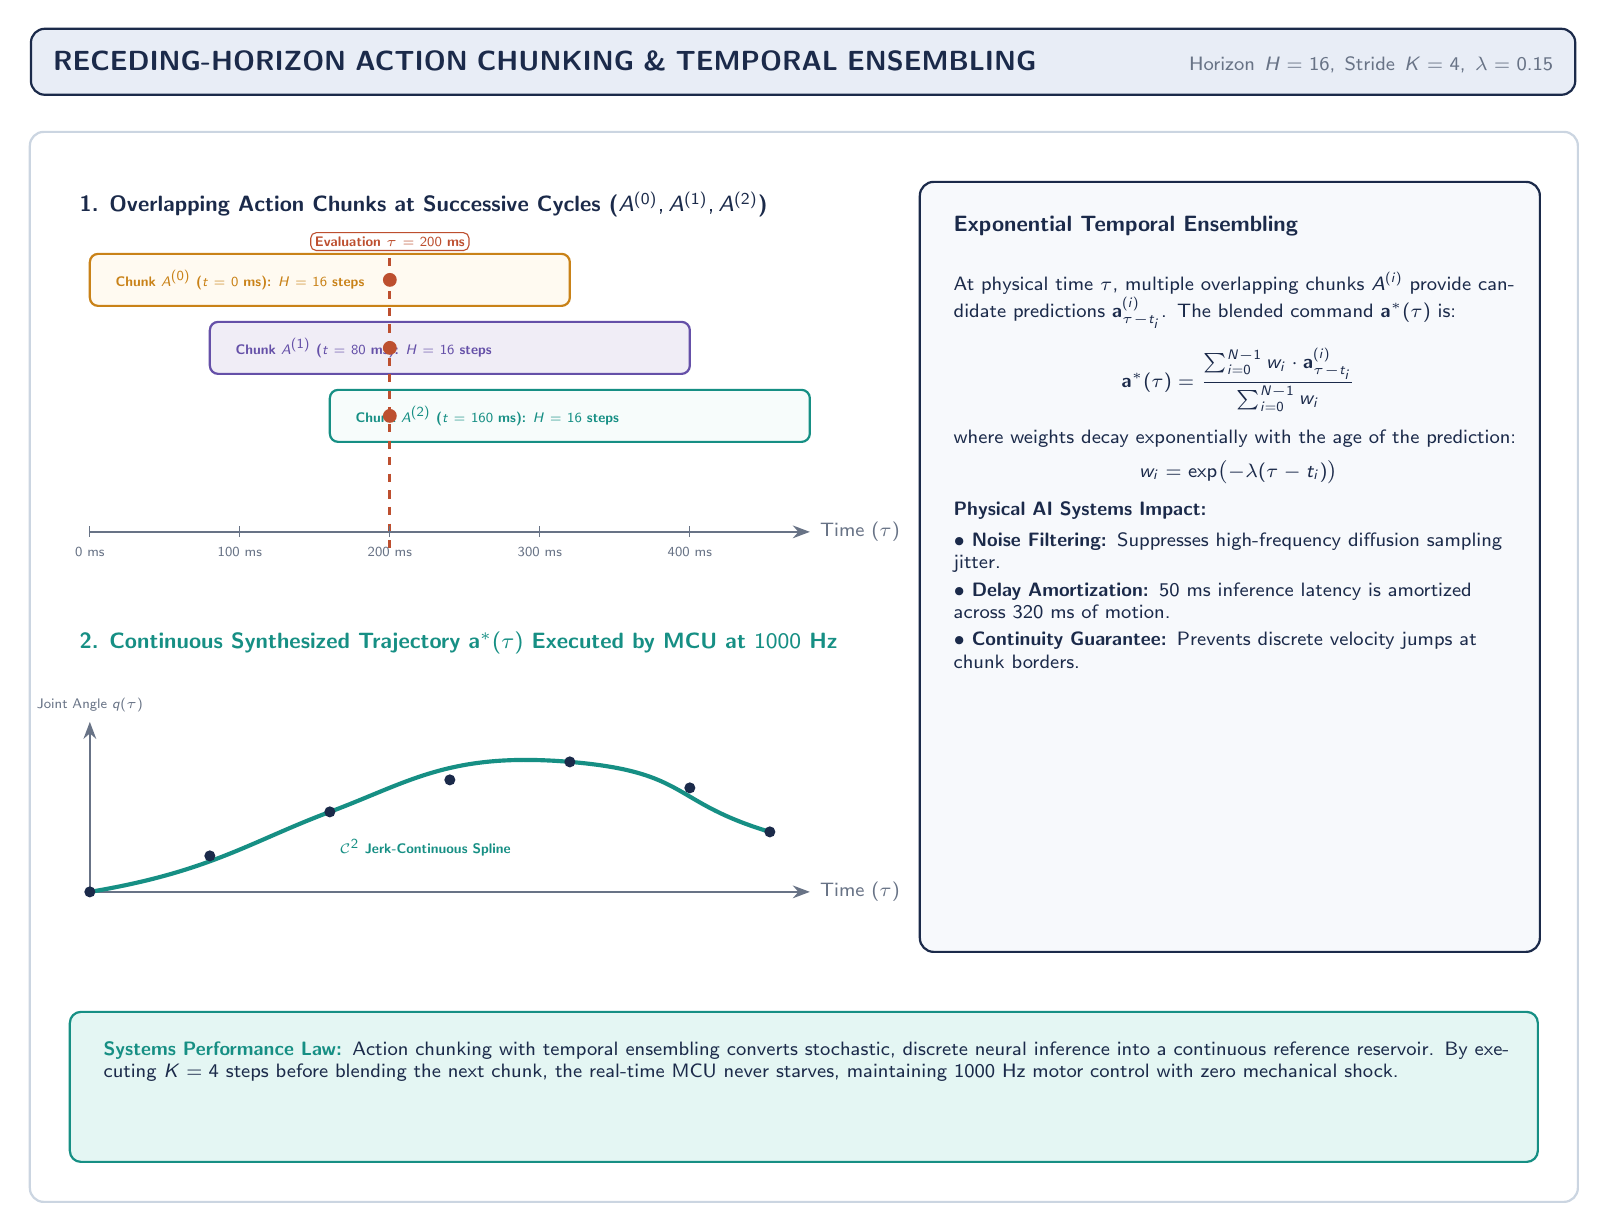
\begin{tikzpicture}[
  font=\sffamily,
  >=Stealth,
  card/.style={
    draw=cardborder,
    fill=white,
    rounded corners=5pt,
    line width=0.8pt,
    inner sep=8pt
  }
]

  % Header Card
  \node[card, fill=navyfill, draw=structuralnavy, text width=7.5in, align=left] (header) {
    \textbf{\color{structuralnavy} RECEDING-HORIZON ACTION CHUNKING \& TEMPORAL ENSEMBLING} \hfill {\scriptsize\color{neutralgray} Horizon $H=16$, Stride $K=4$, $\lambda=0.15$}
  };

  % Main container card
  \coordinate (c_top) at ($(header.south west) + (0, -0.18in)$);
  \draw[draw=cardborder, fill=white, rounded corners=5pt, line width=0.8pt] 
    (c_top) rectangle ++(7.74in, -5.35in);

  % ----------------------------------------------------
  % LEFT COLUMN: The Timing & Splines (Width ~4.2 in)
  % ----------------------------------------------------

  % Section 1 Header
  \coordinate (s1_pos) at ($(c_top) + (0.2in, -0.25in)$);
  \node[anchor=north west, font=\footnotesize\bfseries, color=structuralnavy] at (s1_pos) {
    1. Overlapping Action Chunks at Successive Cycles ($A^{(0)}, A^{(1)}, A^{(2)}$)
  };

  % Chunk 0: emitted at 0ms, spans 16 steps (320ms = 2.4in)
  \draw[draw=proposalamber, fill=amberfill!40, line width=0.8pt, rounded corners=3pt]
    ($(s1_pos) + (0.1in, -0.62in)$) rectangle ++(2.4in, 0.26in);
  \node[anchor=west, font=\tiny\bfseries, color=proposalamber] at ($(s1_pos) + (0.18in, -0.49in)$) {
     Chunk $A^{(0)}$ ($t=0\text{ ms}$): $H=16$ steps
  };

  % Chunk 1: emitted at 80ms (0.6in), spans 2.4in
  \draw[draw=authorityviolet, fill=authorityviolet!10, line width=0.8pt, rounded corners=3pt]
    ($(s1_pos) + (0.7in, -0.96in)$) rectangle ++(2.4in, 0.26in);
  \node[anchor=west, font=\tiny\bfseries, color=authorityviolet] at ($(s1_pos) + (0.78in, -0.83in)$) {
     Chunk $A^{(1)}$ ($t=80\text{ ms}$): $H=16$ steps
  };

  % Chunk 2: emitted at 160ms (1.2in), spans 2.4in
  \draw[draw=measuredteal, fill=tealfill!30, line width=0.8pt, rounded corners=3pt]
    ($(s1_pos) + (1.3in, -1.30in)$) rectangle ++(2.4in, 0.26in);
  \node[anchor=west, font=\tiny\bfseries, color=measuredteal] at ($(s1_pos) + (1.38in, -1.17in)$) {
     Chunk $A^{(2)}$ ($t=160\text{ ms}$): $H=16$ steps
  };

  % Evaluation line at tau = 200ms (1.5in from t0)
  \draw[dashed, line width=1.0pt, consequencecoral] 
    ($(s1_pos) + (1.6in, -0.38in)$) -- ($(s1_pos) + (1.6in, -1.85in)$);
  \node[above=1pt, font=\tiny\bfseries, fill=white, draw=consequencecoral, rounded corners=2pt, inner sep=1.5pt, text=consequencecoral] 
    at ($(s1_pos) + (1.6in, -0.36in)$) {Evaluation $\tau = 200\text{ ms}$};

  % Dots on the chunks at tau = 200ms
  \fill[consequencecoral] ($(s1_pos) + (1.6in, -0.49in)$) circle (2.5pt);
  \fill[consequencecoral] ($(s1_pos) + (1.6in, -0.83in)$) circle (2.5pt);
  \fill[consequencecoral] ($(s1_pos) + (1.6in, -1.17in)$) circle (2.5pt);

  % Timeline Axis 1
  \coordinate (axis1_pos) at ($(s1_pos) + (0.1in, -1.75in)$);
  \draw[->, line width=0.7pt, neutralgray] (axis1_pos) -- ++(3.6in, 0) node[right, font=\scriptsize] {Time ($\tau$)};
  \foreach \x/\label in {0/0, 0.75/100, 1.5/200, 2.25/300, 3.0/400} {
    \draw[neutralgray] ($(axis1_pos) + (\x in, 2pt)$) -- ($(axis1_pos) + (\x in, -2pt)$)
      node[below, font=\tiny] {\label$\text{ ms}$};
  }

  % Section 2 Header (Synthesized Trajectory)
  \coordinate (s2_pos) at ($(c_top) + (0.2in, -2.45in)$);
  \node[anchor=north west, font=\footnotesize\bfseries, color=measuredteal] at (s2_pos) {
    2. Continuous Synthesized Trajectory $\mathbf{a}^*(\tau)$ Executed by MCU at $1000\text{ Hz}$
  };

  % Spline Waveform Axis
  \coordinate (axis2_pos) at ($(s2_pos) + (0.1in, -1.35in)$);
  \draw[->, line width=0.7pt, neutralgray] (axis2_pos) -- ++(3.6in, 0) node[right, font=\scriptsize] {Time ($\tau$)};
  \draw[->, line width=0.7pt, neutralgray] (axis2_pos) -- ++(0, 0.85in) node[above, font=\tiny] {Joint Angle $q(\tau)$};

  % Smooth Spline curve
  \draw[line width=1.5pt, measuredteal] 
    (axis2_pos) .. controls ++(0.6in, 0.1in) and ++(-0.4in, -0.15in) .. 
    ($(axis2_pos) + (1.2in, 0.40in)$) .. controls ++(0.4in, 0.15in) and ++(-0.6in, 0.05in) .. 
    ($(axis2_pos) + (2.4in, 0.65in)$) .. controls ++(0.6in, -0.05in) and ++(-0.5in, 0.15in) .. 
    ($(axis2_pos) + (3.4in, 0.30in)$);

  % Waypoints
  \foreach \x/\y in {0/0, 0.6/0.18, 1.2/0.40, 1.8/0.56, 2.4/0.65, 3.0/0.52, 3.4/0.30} {
    \fill[structuralnavy] ($(axis2_pos) + (\x in, \y in)$) circle (2pt);
  }
  \node[anchor=west, font=\tiny\bfseries, color=measuredteal] at ($(axis2_pos) + (1.2in, 0.22in)$) {
    $\mathcal{C}^2$ Jerk-Continuous Spline
  };

  % ----------------------------------------------------
  % RIGHT COLUMN: Mathematical Formulation Box
  % ----------------------------------------------------
  \coordinate (rbox_pos) at ($(c_top) + (4.45in, -0.25in)$);
  \draw[draw=structuralnavy, fill=navyfill!35, rounded corners=5pt, line width=0.8pt]
    (rbox_pos) rectangle ++(3.1in, -3.85in);

  \node[anchor=north west, font=\footnotesize\bfseries, color=structuralnavy] at ($(rbox_pos) + (0.12in, -0.12in)$) {
     Exponential Temporal Ensembling
  };

  \node[anchor=north west, font=\scriptsize, text width=2.85in, align=left, color=structuralnavy] at ($(rbox_pos) + (0.12in, -0.40in)$) {
    At physical time $\tau$, multiple overlapping chunks $A^{(i)}$ provide candidate predictions $\mathbf{a}_{\tau - t_i}^{(i)}$. The blended command $\mathbf{a}^*(\tau)$ is:
    \\[6pt]
    \centering
    $\mathbf{a}^*(\tau) = \dfrac{\sum_{i=0}^{N-1} w_i \cdot \mathbf{a}_{\tau - t_i}^{(i)}}{\sum_{i=0}^{N-1} w_i}$
    \\[6pt]
    \raggedright
    where weights decay exponentially with the age of the prediction:
    \\[4pt]
    \centering
    $w_i = \exp\bigl(-\lambda (\tau - t_i)\bigr)$
    \\[6pt]
    \raggedright
    \textbf{Physical AI Systems Impact:}\\[3pt]
    $\bullet$ \textbf{Noise Filtering:} Suppresses high-frequency diffusion sampling jitter.\\[2pt]
    $\bullet$ \textbf{Delay Amortization:} $50\text{ ms}$ inference latency is amortized across $320\text{ ms}$ of motion.\\[2pt]
    $\bullet$ \textbf{Continuity Guarantee:} Prevents discrete velocity jumps at chunk borders.
  };

  % ----------------------------------------------------
  % BOTTOM TAKEAWAY BANNER (Inside container)
  % ----------------------------------------------------
  \coordinate (bot_pos) at ($(c_top) + (0.2in, -4.40in)$);
  \draw[draw=measuredteal, fill=tealfill, rounded corners=4pt, line width=0.8pt]
    (bot_pos) rectangle ++(7.34in, -0.75in);

  \node[anchor=north west, font=\scriptsize, text width=7.15in, align=left, color=structuralnavy] at ($(bot_pos) + (0.12in, -0.10in)$) {
    \textbf{\color{measuredteal} Systems Performance Law:} Action chunking with temporal ensembling converts stochastic, discrete neural inference into a continuous reference reservoir. By executing $K=4$ steps before blending the next chunk, the real-time MCU never starves, maintaining $1000\text{ Hz}$ motor control with zero mechanical shock.
  };

\end{tikzpicture}
\end{document}
